\documentclass[aspectratio=169]{beamer}
\usetheme{Bruno}
\usepackage{amsmath}
\usepackage{amssymb}
\usepackage{siunitx}
\usepackage{float}
\usepackage{tikz}
\def\checkmark{\tikz\fill[scale=0.4](0,.35) -- (.25,0) -- (1,.7) -- (.25,.15) -- cycle;} 
\usepackage{url}
\usepackage[siunitx,american,RPvoltages]{circuitikz}
\ctikzset{capacitors/scale=0.7}
\ctikzset{diodes/scale=0.7}
\usepackage{tabularx}
\newcolumntype{C}{>{\centering\arraybackslash}X}
\renewcommand\tabularxcolumn[1]{m{#1}}% for vertical centering text in X column
\usepackage{tabu}
\usepackage[spanish,es-tabla,activeacute]{babel}
\usepackage{babelbib}
\usepackage{booktabs}
\usepackage{pgfplots}
\usepackage{hyperref}
\hypersetup{colorlinks = true,
            linkcolor = black,
            urlcolor  = blue,
            citecolor = blue,
            anchorcolor = blue}
\usepgfplotslibrary{units, fillbetween} 
\pgfplotsset{compat=1.16}
\usepackage{bm}
\usetikzlibrary{arrows, arrows.meta, shapes, 3d, perspective, positioning,mindmap,trees,backgrounds}
\renewcommand{\sin}{\sen} %change from sin to sen
\usepackage{bohr}
\setbohr{distribution-method = quantum,insert-missing = true}
\usepackage{elements}
\usepackage{verbatim}
\usepackage[edges]{forest}
\usepackage{etoolbox}
\usepackage{schemata}
\usepackage{appendix}
\usepackage{listings}

\definecolor{color_mate}{RGB}{255,255,128}
\definecolor{color_plas}{RGB}{255,128,255}
\definecolor{color_text}{RGB}{128,255,255}
\definecolor{color_petr}{RGB}{255,192,192}
\definecolor{color_made}{RGB}{192,255,192}
\definecolor{color_meta}{RGB}{192,192,255}
\newcommand\diagram[2]{\schema{\schemabox{#1}}{\schemabox{#2}}}

\definecolor{codegreen}{rgb}{0,0.6,0}
\definecolor{codegray}{rgb}{0.5,0.5,0.5}
\definecolor{codepurple}{rgb}{0.58,0,0.82}
\definecolor{backcolour}{rgb}{0.95,0.95,0.92}

\lstdefinestyle{mystyle}{
    backgroundcolor=\color{backcolour},   
    commentstyle=\color{codegreen},
    keywordstyle=\color{magenta},
    numberstyle=\tiny\color{codegray},
    stringstyle=\color{codepurple},
    basicstyle=\ttfamily\footnotesize,
    breakatwhitespace=false,         
    breaklines=true,                 
    captionpos=b,                    
    keepspaces=true,                 
    numbers=left,                    
    numbersep=5pt,                  
    showspaces=false,                
    showstringspaces=false,
    showtabs=false,                  
    tabsize=2
}

\lstset{style=mystyle}
\title{Instrumentación I: \\ \emph{Medidas de nivel}}
\author{
    Juan J. Rojas, Hugo Sanchez Ortiz
}
\institute{Instituto Tecnológico de Costa Rica}
\date{\today}
\background{fig/background.jpg}
\begin{document}
\sisetup{unit-math-rm=\mathrm,math-rm=\mathrm} % change sinitx font
\sisetup{output-decimal-marker = {,}}
\maketitle

\newcommand{\blackandwhite}{white} %change this at the end

\begin{frame}{Definiciones}
    \begin{columns}[c, onlytextwidth]
        \begin{column}{0.45\textwidth}
            \begin{itemize}
                \item En la industria existe una clara necesidad del manejo y control de materias primas. Lo cual permite un balance y una organización de la producción.
                \item Sin importar el material (agua, petroléo, sodio), estas mediciones permiten garantizar la seguridad 
                \item Accidentes como  \href{https://www.bbc.com/news/uk-10266706}{la explosión masiva de la Terminal de Petroleo de Buncefield, UK}, se debió a la mala medición de nivel. 
            \end{itemize}
        \end{column}
        \begin{column}{0.50\textwidth}
            \includegraphics[width = 1\linewidth]{fig/Nivel/Introducción.jpg}
            
            \tiny{\href{https://www.predig.com/whitepaper/level-measurement-technologies-process-control-industry}{By: Precision Digital}}
        \end{column}
    \end{columns}
\end{frame}

\begin{frame}{Tipos de Medición}
    \begin{columns}[c, onlytextwidth]
        \begin{column}{0.45\textwidth}
        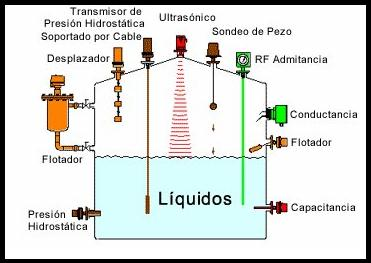
\includegraphics[width = 1\linewidth]{fig/Nivel/Nivel-de-liquidos.png}
        \tiny{Tomado de \cite{sole2005instrumentacion}}
        \end{column}
        \begin{column}{0.50\textwidth}
            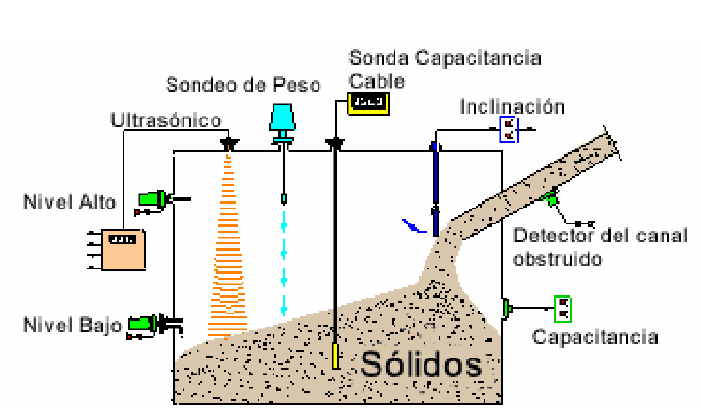
\includegraphics[width = 1\linewidth]{fig/Nivel/Nivel-de-solidos.png}
        \end{column}
    \end{columns}
\end{frame}

\begin{frame}{Tecnologías de Medición}

 \begin{columns}[c, onlytextwidth]
        \begin{column}{0.40\textwidth}
        \centering
            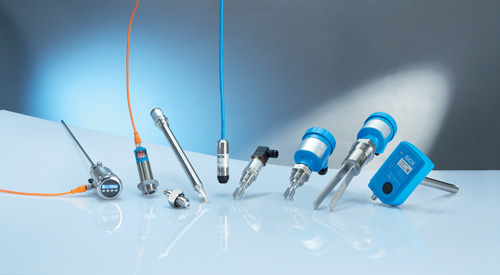
\includegraphics[width=6.5cm]{fig/Nivel/level-sensors.jpg}
            \\ \tiny{Tomado de \href{https://sickusablog.com/level-measurement-choosing-right-sensor/}{aquí}}
        \end{column}
        \begin{column}{0.50\textwidth}
               \centering
    \diagram{Tecnologías}
        {- Medida Directa \\
        - Presión hidróstatica \\
        - Basado en el desplazamiento\\
        - Características Eléctricas\\
        - Medidor Ultrasónico\\
        - Radar o Microondas\\
        - Nivel de Radiación\\
        - De Láser\\
        - Vibración\\
        }
        \end{column}
    \end{columns}


\end{frame}

\begin{frame}{Tecnologías de Medición}
\begin{table}
 \small
    \centering
    \begin{tabular}{m{3.2cm} m{1.2cm} m{2.6cm} m{2.6cm} m{1.8cm} m{2cm}}
        \toprule
        \textbf{Tipo de Sensor} & \textbf{Líquidos} & \textbf{Sólidos} &\textbf{Fluidos Viscosos}\\
        \midrule
        \textbf{Laser} & \textcolor{green}{\checkmark}  & \textcolor{green}{\checkmark} & Depende del material \\
        \textbf{Ultrasónico} & \textcolor{green}{\checkmark} & \textcolor{green}{\checkmark} & \textcolor{red}{X} \\
        \textbf{Óptico} & \textcolor{green}{\checkmark} & \textcolor{red}{X} & \textcolor{red}{X}\\
        \textbf{Presión hidrostática} & \textcolor{green}{\checkmark} & \textcolor{red}{X} & \textcolor{red}{X} \\
        \textbf{Capacitancia} & \textcolor{green}{\checkmark} & Depende del material & \textcolor{red}{X} \\
        \textbf{Flotador} & \textcolor{green}{\checkmark} & \textcolor{red}{X} & Depende del material \\
        \textbf{Radar o Microondas} & \textcolor{green}{\checkmark} & \textcolor{green}{\checkmark} & \textcolor{green}{\checkmark} \\
        \bottomrule
    \end{tabular}
    \caption{Comparación entre distintos tipos de presión electrónicos de vacío} \cite{pallas2012sensors}
    \label{tab:Comparacionvacio}
\end{table}
\end{frame}

\begin{frame}{Instrumentos de medición directa}
    \begin{columns}[c, onlytextwidth]
        \begin{column}{0.45\textwidth}
        \textbf{Medidor de sonda}
            \begin{itemize}
                \item El medidor de sonda consiste en una varilla que se ingresa dentro del recipiente. 
                \item La medición se realiza mediante una lectura directa.  
                \item En el momento de lectura el tanque deberá estar abierto a presión atmósferica.
            \end{itemize}
        \end{column}
        \begin{column}{0.50\textwidth}
            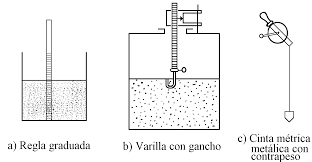
\includegraphics[width = 1.1\linewidth]{fig/Nivel/MedicionSonda.png}
            \tiny{Tomado de \cite{sole2005instrumentacion}}
        \end{column}
    \end{columns}
\end{frame}

\begin{frame}{Instrumentos de medición directa}
    \begin{columns}[c, onlytextwidth]
        \begin{column}{0.45\textwidth}
        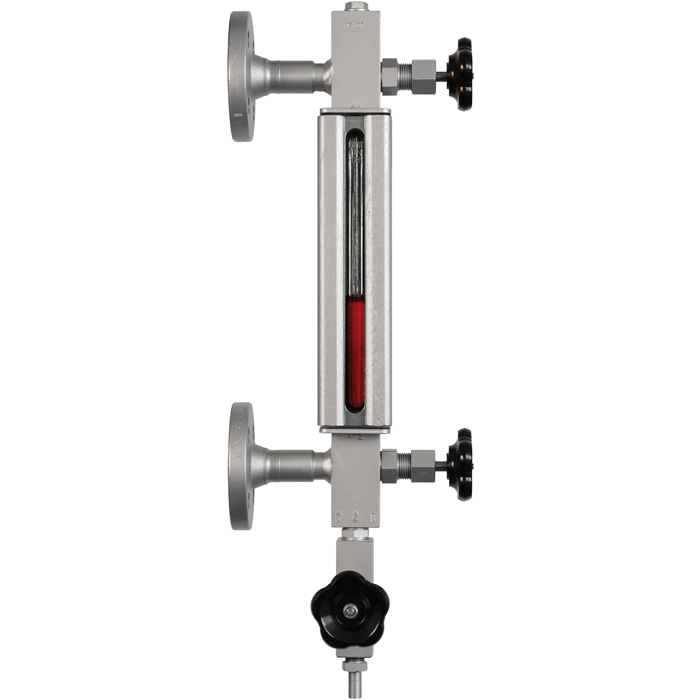
\includegraphics[width = 1\linewidth]{fig/Nivel/medidor_cristal.png}
            %\tiny{Tomado de \cite{sole2005instrumentacion}}
        \end{column}
        \begin{column}{0.50\textwidth}
        \textbf{Medidor de cristal}
            \begin{itemize}
                \item Es un tubo de vidrio conectado a bloques, que se encuentran unidos mediante tres válvulas.
                \item Se emplea para medir presiones de hasta 7 bar. Si se requieren mayor medir mayor presión, es necesario engrosar las paredes.   
                \item ofrecen es la gran seguridad que ofrece en la lectura del nivel del líquido pudiendo controlar con ellos la lectura de los otros aparatos de nivel.
                \item Se pueden utilizar reflectores.
            \end{itemize}
            
        \end{column}
    \end{columns}
\end{frame}

\begin{frame}{Instrumentos de medición directa}
    \begin{columns}[c, onlytextwidth]
        \begin{column}{0.45\textwidth}
        \textbf{Flotadores}
            \begin{itemize}
                \item Consiste en un flotador situado en la superficie del líquido, con un indicador externo al tanque. 
                \item Existen mediciones directas, magnéticas e hidráulicas  
                \item Sustituyen a los de vidrio cuando: 
                \begin{itemize}
                    \item La presión es superior a 25 bar. 
                    \item Posibilidad de ruptura al vidrio.
                    \item Evitar escape de líquidos o gases. 
                    \item Depósitos enterrados. 
                \end{itemize}
            \end{itemize}
        \end{column}
        \begin{column}{0.50\textwidth}
            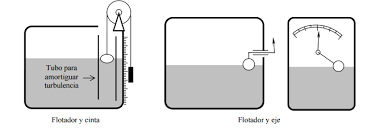
\includegraphics[width = 1.1\linewidth]{fig/Nivel/flotador.png}
            \tiny{Tomado de \cite{sole2005instrumentacion}}
        \end{column}
    \end{columns}
\end{frame}

            

\begin{frame}{Instrumentos de medición directa}
    \begin{columns}[c, onlytextwidth]
        \begin{column}{0.45\textwidth}
        \centering
        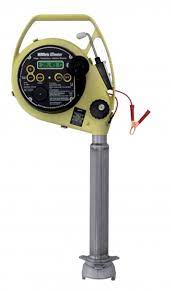
\includegraphics[width = 0.6\linewidth]{fig/Nivel/Servooperado.jpg}
            \tiny{\href{https://www.emerson.com}{By: Emerson}}
        \end{column}
        \begin{column}{0.55\textwidth}
        \textbf{Medidor de palpador servooperado}
            \begin{itemize}
                \item Un disco de desplazamiento suspendido por una cinta perforada, acoplada a un tambor ranurado.
                \item Cuando el nivel del producto cambia, el desplazador es cambia automáticamente manteniendo el contacto con la superficie del producto.   
                \item Está montado en el techo del tanque y dispone de un codificador óptico y del transmisor de los datos de nivel.
                \item Exactitud de ± 3 mm, y un campo de medida de 1 mm a 30 m.
            \end{itemize}
            
        \end{column}
    \end{columns}
\end{frame} 

\begin{frame}{Instrumentos de medición directa}
    \begin{columns}[c, onlytextwidth]
        \begin{column}{0.45\textwidth}
        \textbf{Nivel magnoestrictivo}
            \begin{itemize}
                \item Utiliza un flotador cuya posición se determina mediante el fenómeno de magnetoestrición.  
                \item mide el intervalo de tiempo entre el impulso inicial de y el impulso de retorno y lo convierte a una señal dentro del intervalo de 4-20 mA,  
                \item puede utilizarse en la medida de interfases líquido-líquido. La exactitud es del ± 0,01\%. El alcance (\textit{span}) es de 0,1 m a 5 m
            \end{itemize}
        \end{column}
        \begin{column}{0.50\textwidth}
            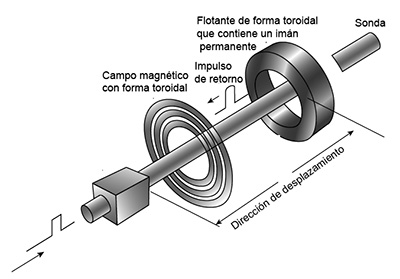
\includegraphics[width = 1.1\linewidth]{fig/Nivel/Magnetostrictivo.jpg}
            \tiny{\href{https://www.kobold.com/uploads/files/n2es_nmt.pdf}{By: Kobold}}
        \end{column}
    \end{columns}
\end{frame}


\begin{frame}{Instrumentos basados en presión hidrostática}
    \begin{columns}[c, onlytextwidth]
        \begin{column}{0.45\textwidth}
        \textbf{Nivel manométrico}
            \begin{itemize}
                \item consiste en un sensor de presión piezoresistivo suspendido de la parte superior del tanque e inmerso en el líquido. 
                \item El sensor contiene un puente de Wheastone
                \item El nivel se mide por: 
                $P=H\times \lambda \times g$
            \end{itemize}
        \end{column}
        \begin{column}{0.50\textwidth}
            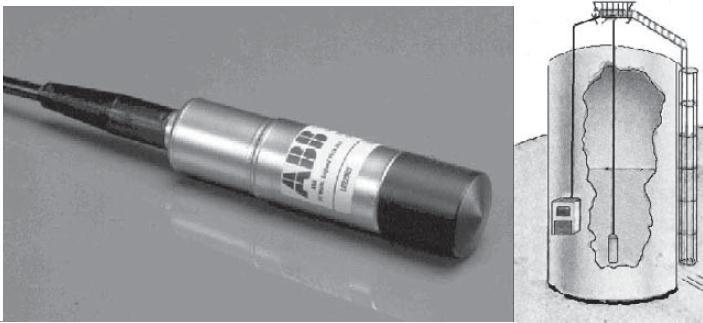
\includegraphics[width = 1.1\linewidth]{fig/Nivel/Manometrico.jpg}
            \tiny{Tomado de \cite{sole2005instrumentacion}}
            \tiny{\href{ https://sai-tech.mx/webpage/category/abb/medicion-y-analiticos/abb-medicion-nivel/}{Medidores ABB}}
           
        \end{column}
    \end{columns}
\end{frame}

\begin{frame}{Instrumentos basados en presión hidrostática}
    \begin{columns}[c, onlytextwidth]
        \begin{column}{0.45\textwidth}
        \centering
        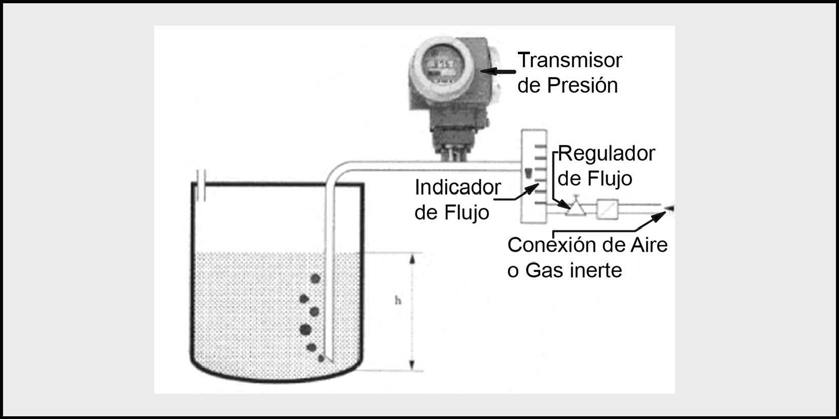
\includegraphics[width = 1\linewidth]{fig/Nivel/Burbujeo.png}
            \tiny{\href{https://www.researchgate.net/publication/316675361_Fundamentos_de_la_medicion_de_presion_nivel_y_caudal_en_los_sistemas_hidraulicos}{Sensores Burbujeo}}
        \end{column}
        \begin{column}{0.55\textwidth}
        \textbf{Medidor de tipo burbujeo}
            \begin{itemize}
                \item Emplea un tubo sumergido en el líquido a cuyo través se hace burbujear aire mediante un rotámetro con un regulador de caudal incorporado
                \item La presión del aire en la tubería equivale a la presión hidrostática ejercida por la columna de líquido, es decir, al nivel. 
                \item El manómetro receptor puede colocarse hasta distancias de 200 m.
    
            \end{itemize}
            
        \end{column}
    \end{columns}
\end{frame} 

\begin{frame}{Instrumentos basados en presión hidrostática}
    \begin{columns}[c, onlytextwidth]
        \begin{column}{0.45\textwidth}
        \textbf{Nivel de presión diferencial}
            \begin{itemize}
                \item consiste en un diafragma en contacto con el líquido que mide la presión hidrostática en un punto del fondo del tanque. En 
                \item En el caso de que el tanque esté cerrado y bajo presión, hay que corregir la indicación del aparato para la presión ejercida sobre el líquido.
            \end{itemize}
        \end{column}
        \begin{column}{0.50\textwidth}
            \includegraphics[width = 1.1\linewidth]{fig/Nivel/Presión diferencial.jpg}           \tiny{\href{https://www.emerson.com/es-es/automation/measurement-instrumentation/pressure-measurement/about-differential-pressure-dp-level-measurement}{By: Emerson}}
           
        \end{column}
    \end{columns}
\end{frame}

\begin{frame}{Instrumentos basados en presión hidrostática}
    \textbf{Medición de interfase de líquidos}
    \centering
    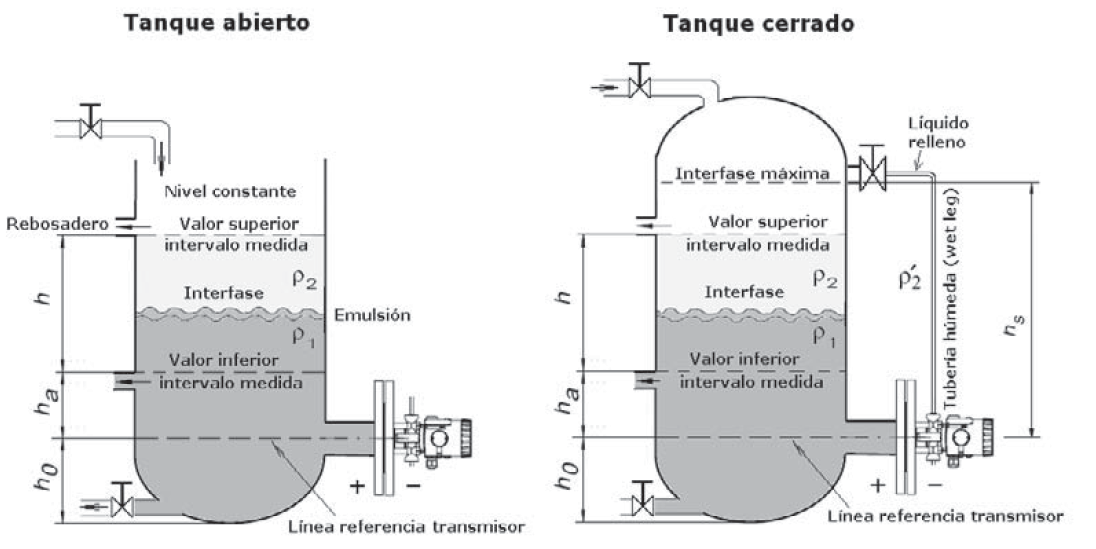
\includegraphics[width = 0.8\linewidth]{fig/Nivel/Interfaz.PNG}\\
            \tiny{Tomado de \cite{sole2005instrumentacion}}
\end{frame}

\begin{frame}{Instrumentos basados en desplazamiento}
    \begin{columns}[c, onlytextwidth]
        \begin{column}{0.45\textwidth}
        \centering
        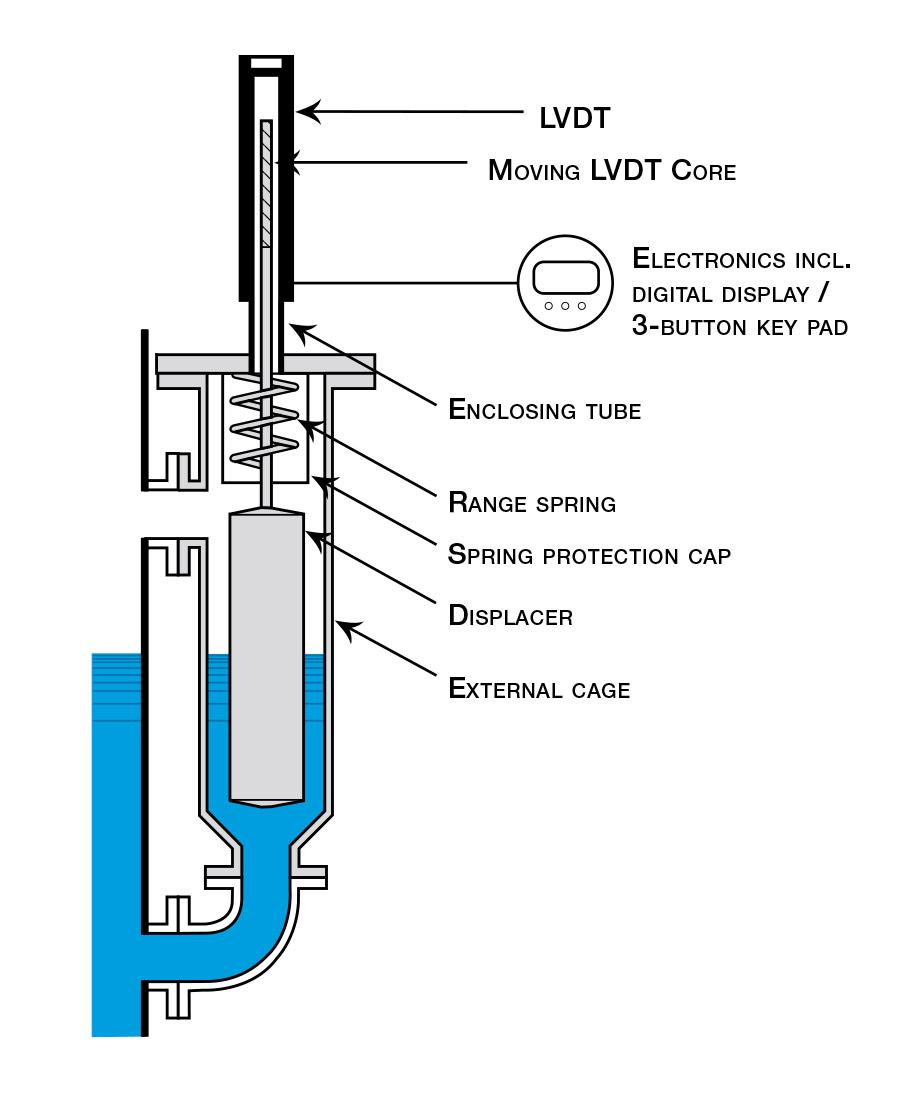
\includegraphics[width = 0.8\linewidth]{fig/Nivel/Desplazamiento.jpg}\\
            \tiny{\href{https://www.magnetrol.com/es/transmisor-de-nivel-por-desplazador}{Transmisor de nivel por desplazamiento}}
        \end{column}
        \begin{column}{0.55\textwidth}
            \begin{itemize}
                \item Consiste en un flotador parcialmente sumergido en el líquido y conectado mediante un brazo a un tubo de torsión unido rígidamente al tanque o bien a un resorte de equilibrio del que pende el flotador.
                \item Se genera una fuerza, mediante el principio: $F=S\times H \times \lambda \times g$ 
                \item Pueden utilizarse en ruidos sucios a altas presiones 170 bar (17 MPa - 2.465 psi) y temperaturas elevadas, desde 200 °C hasta 450 °C.
    
            \end{itemize}
            
        \end{column}
    \end{columns}
\end{frame} 

\begin{frame}{Instrumentos basados en características eléctricas}
    \begin{columns}[c, onlytextwidth]
        \begin{column}{0.5\textwidth}
        \textbf{Conductivo o resistivo}
            \begin{itemize}
                \item consiste en uno o varios electrodos y un circuito electrónico que excita un relé eléctrico o electrónico al ser los electrodos mojados por el líquido.
                \item La impedancia mínima es del orden de los 25 MW/cm
                \item El relé electrónico dispone de un temporizador de retardo que impide su enclavamiento ante una ola del nivel del líquido o ante cualquier perturbación.
            \end{itemize}
        \end{column}
        \begin{column}{0.50\textwidth}
        \centering
            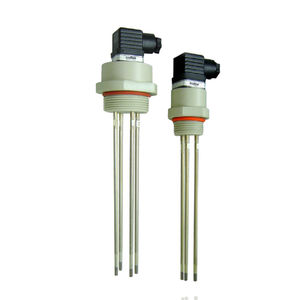
\includegraphics[width = 1.1\linewidth]{fig/Nivel/Resistivo.jpg}           \tiny{\href{http://www.divatecsl.com/productos/interruptor-nivel-conductivo-cfp/}{By: Divatec}}
           
        \end{column}
    \end{columns}
\end{frame}

\begin{frame}{Instrumentos basados en características eléctricas}
    \begin{columns}[c, onlytextwidth]
        \begin{column}{0.5\textwidth}
                \centering
            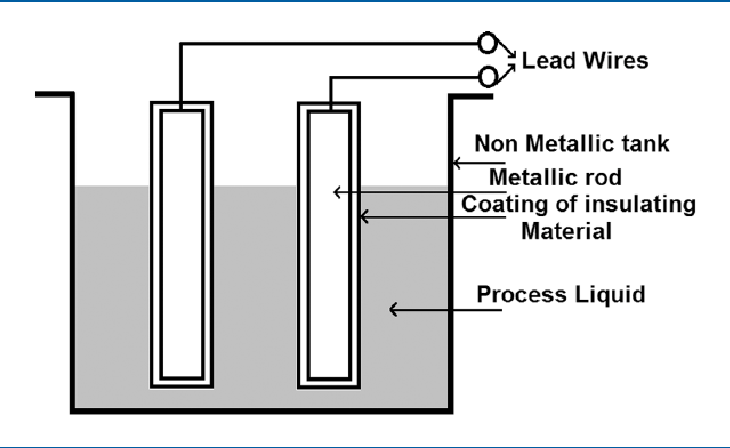
\includegraphics[width = 0.9\linewidth]{fig/Nivel/capacitance.png}\\           \tiny{\href{https://www.semanticscholar.org/paper/A-Review-on-Capacitive-Type-Sensor-for-Measurement-Kumar-Rajita/2e3d6ede8338e72be9972741eafed7f50388b53a}{A Review on Capacitive-Type Sensor for Measurement of Height of Liquid Level}}
        \end{column}
        \begin{column}{0.50\textwidth}
        
        \textbf{Capacitivo}
            \begin{itemize}
                \item Mide la capacidad del condensador formado por un electrodo sumergido en el líquido y las paredes del tanque.
                \item Trabaja en la gama baja de radiofrecuencia de pocos MHz, midiendo la admitancia de un circuito de corriente alterna, la que varía según el nivel de líquido en el tanque.
            \end{itemize}
        
        \end{column}
    \end{columns}
\end{frame}

\begin{frame}{Constantes dieléctricas de varios tipos de materiales}
    \begin{columns}[c, onlytextwidth]
        \begin{column}{0.5\textwidth}
        \textbf{Capacitivo}
            \begin{itemize}
                \item La formula de capacitancia está dada por:\\ $C=K\times \frac{A}{D}$
                \item La impedancia del sistema está dado por: \\
                $Z=R+\frac{1}{\sqrt{2\pi \times f \times C}}$
                \item La distancia entre el electrodo y las paredes del tanque y el área de los conductores permanecen constantes. 
            \end{itemize}
        \end{column}
        \begin{column}{0.50\textwidth}
        \centering
            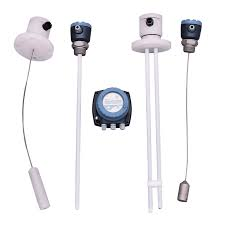
\includegraphics[width = 0.9\linewidth]{fig/Nivel/capacitance_types.png} \\          \tiny{\href{https://www.toshbrocontrols.com/level-transmitter/rf-capacitance-level-transmitter}{By: Toshbrocontrols}}
           
        \end{column}
    \end{columns}
\end{frame}

\begin{frame}{Constantes dieléctricas de varios tipos de materiales}
 \begin{table}[]
 \footnotesize
    \centering
    \begin{tabular}{m{1.8cm} m{0.8cm} m{1.8cm} m{0.8cm} m{0.8cm} m{1.8cm} m{0.8cm} m{0.8cm} m{1.6cm}}
        \toprule
        \textbf{Sólido}  & \textbf{K} &\textbf{Líquido} & \textbf{$^\circ C$} & \textbf{K} &\textbf{Líquido} & \textbf{$^\circ C$} & \textbf{K} \\
        \midrule
        \textbf{Asbesto} & 4.8 & \textbf{Acetona} & 22 & 21.4 &  \textbf{Heptano} & 20  & 1.9\\
        \textbf{Asfalto} & 2.7 & \textbf{Amoníaco} & -33 & 22.4 & \textbf{Keroseno} & 21 & 1.8\\
        \textbf{Nylon} & 45 & \textbf{Benceno} & 20 & 2.3 & \textbf{Octano} & 20 & 2.0\\
       \textbf{Polyetileno} & 4.5 &  \textbf{Butano} & -1 & 1.4 & \textbf{Sulfuro} & 400 & 3.4\\
        \textbf{Porcelana} & 5.7 & \textbf{Etanol} & 25 & 24.3 & \textbf{Uretano} & 23 & 23\\
        \textbf{Arena} & 3.5 & \textbf{Etyl Acetato} & 20 & 6.4 & \textbf{Agua} & 80 & 80\\
        \textbf{Azúcar} & 3 & \textbf{Glycol} & 20 & 41.2 & \textbf{Agua} & 100 & 48\\
        \bottomrule
    \end{tabular}
    \caption{Constantes dieléctricas para varios materiales \cite{sole2005instrumentacion}}
    \label{tab:Comparacion}
\end{table}
\end{frame}

\begin{frame}{Medidores de nivel por ultrasonido}
    \begin{columns}[c, onlytextwidth]
        \begin{column}{0.5\textwidth}
                
            \begin{itemize}
                \item se basa en la emisión de un impulso ultrasónico a una superficie reflectante y la recepción del eco del mismo en un receptor. El retardo en la captación del eco depende del nivel del tanque.
                \item El nivel del tanque está dado por:\\
                $h=\frac{v \times t}{2}$
                \item la aplicación típica es situar el emisor en la parte superior del tanque y dirigir el impulso ultrasónico a la superficie del líquido para ser reflejado y retornar al receptor.
            \end{itemize}
                
        \end{column}
        \begin{column}{0.50\textwidth}
        \centering
            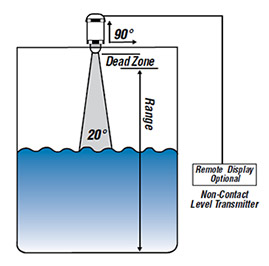
\includegraphics[width = 0.8\linewidth]{fig/Nivel/ultrasonic.jpg}\\
            \tiny{\href{https://es.omega.com/technical-learning/transmisores-flujo-nivel-monitoreo-presion-recipiente.html}{By: Omega Engineering}}
        \end{column}
    \end{columns}
\end{frame}

\begin{frame}{Medidores de radar o microondas}
    \begin{columns}[c, onlytextwidth]
        \begin{column}{0.5\textwidth}
                \centering
            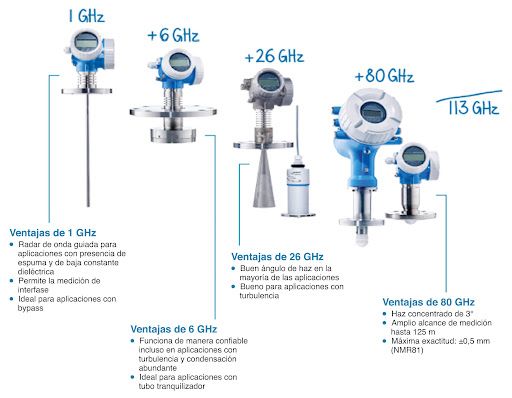
\includegraphics[width = 0.9\linewidth]{fig/Nivel/radar}\\           \tiny{\href{http://www.edcontrol.com/index.php/instrumentacion/item/12-confusion-en-el-mundo-de-las-mediciones-de-nivel-por-radar-no-es-para-tanto}{Técnicas de radar}}
        \end{column}
        \begin{column}{0.50\textwidth}
        
            \begin{itemize}
                \item El sensor está situado en la parte superior del tanque y envía las microondas hacia la superficie del líquido. Una parte de la energía enviada es reflejada en la superficie del líquido y la capta el sensor.
                \item $D=\frac{(v \times t)}{2}$ y $v=\frac{c}{\sqrt{e}}$
                \item Si la constante dieléctrica del líquido es baja, pueden presentarse problemas en la medida.
                
            \end{itemize}
        
        \end{column}
    \end{columns}
\end{frame}

\begin{frame}{Medidores de nivel por radiación}
    \begin{columns}[c, onlytextwidth]
        \begin{column}{0.5\textwidth}
                
            \begin{itemize}
                \item Consiste en un emisor de rayos gamma montado verticalmente en un lado del tanque y con un contador Geiger que transforma la radiación gamma recibida en una señal eléctrica de corriente continua
                \item Como la transmisión de los rayos es inversamente proporcional a la masa del líquido en el tanque, la radiación captada por el receptor es inversamente proporcional al nivel del líquido.
                
            \end{itemize}
                
        \end{column}
        \begin{column}{0.50\textwidth}
        \centering
            \includegraphics[width = 0.8\linewidth]{fig/Nivel/radiación.png}\\
            \tiny{Tomado de \cite{sole2005instrumentacion}}
        \end{column}
    \end{columns}
\end{frame}

\begin{frame}{Medidores de nivel láser}
    \begin{columns}[c, onlytextwidth]
        \begin{column}{0.5\textwidth}
                \centering
            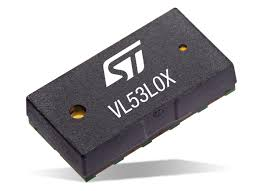
\includegraphics[width = 0.9\linewidth]{fig/Nivel/lasersensor.jpg}\\           \tiny{\href{https://www.mouser.com/new/stmicroelectronics/stm-vl53lox-sensor/}{STMicroelectronics VL53L0X Time-of-Flight Ranging Sensor}}
        \end{column}
        \begin{column}{0.50\textwidth}
        
            \begin{itemize}
                \item Consiste en un rayo láser (Light Amplification by Stimulated Emission of Radiation) enviado a través de un tubo de acero y dirigido por reflexión en un espejo.
                \item $D=\frac{(C \times t)}{2}$.
                \item La velocidad en la toma de datos del nivel puede llegar a ser de 3 lecturas por segundo.
                
            \end{itemize}
        
        \end{column}
    \end{columns}
\end{frame}

\begin{frame}{Medidores de nivel de líquidos}
 \begin{table}[]
 \footnotesize
    \centering
    \begin{tabular}{m{3.2cm} m{1.2cm} m{1.2cm} m{1.9cm} m{1.8cm} m{1.6cm}}
        \toprule
        \textbf{Tipo de Sensor} & \textbf{Campo medida} & \textbf{Exactitud [$\%$]} &\textbf{P. Máx. [bar]} & \textbf{Temperatura [$^{\circ}C$]} & \textbf{Precio} \\
        \midrule
        \textbf{Sonda} & Limitado & 0.5 mm & 1 atm & 60 & Bajo\\
        \textbf{Flotador} & 0-10m & $\pm1-2\%$ & 400 & 250 & Bajo\\
        \textbf{Manométrico} & Tanque & $\pm1\%$ & 1 atm & 60 & Bajo\\
        \textbf{Burbujeo} & Tanque & $\pm1\%$ & 1 atm & 200  & Bajo\\
        \textbf{Diferencial} & 0-10m & $\pm0.1\%$ & 150 & 600  & Medio\\
        \textbf{Desplazamiento} & 0-25m & $\pm0.5\%$ & 100 & 400 & Medio\\
        \textbf{Conductivo} & Limitado & $\pm 3 mm$ & 80 & 800 & Bajo\\
        \textbf{Capacitivo} & 0-6m & $\pm 1\%$ & 250 & 800 & Medio\\
        \textbf{Ultrasónico} & 0-3m & $\pm 1\%$ & 400 & 200 & Alto\\
        \textbf{Radar} & 0-30m & $\pm 2,5 mm$ & - & 230 & Alto\\
        \textbf{Radiación} & 0-2.5m & $\pm0.5\%$ & - & 150 & Alto\\
        \textbf{Láser} & Limitado & $\pm0.5\%$ &    -& 1500 & Alto\\
        \textbf{Vibratorio} & Limitado & $\pm 5 mm$ &  & 150 & Bajo\\
        \bottomrule
    \end{tabular}
    \tiny{\caption{Comparación entre distintos medidores de nivel de líquidos} \cite{sole2005instrumentacion}}
    \label{tab:Comparacion_sensores}
\end{table}
\end{frame}

\begin{frame}{Medidores de nivel de sólidos (punto fijo)}
    \begin{columns}[c, onlytextwidth]
        \begin{column}{0.45\textwidth}
        \textbf{Diafragmas}
            \begin{itemize}
                \item Consiste en una membrana flexible que puede entrar en contacto con el producto dentro del tanque y que actúa sobre un microrruptor.
                \item El material del diafragma puede ser de tela, goma, neopreno o fibra de vidrio. 
                \item La exactitud es de ± 50 mm.
            \end{itemize}
        \end{column}
        \begin{column}{0.50\textwidth}
        \centering
            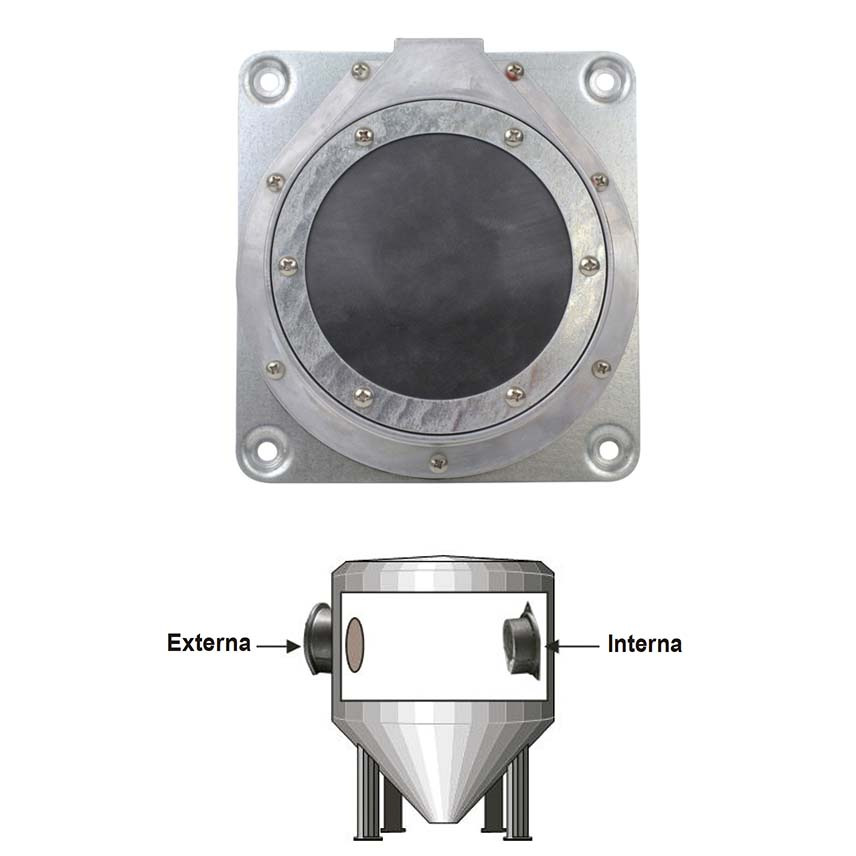
\includegraphics[width = 0.8\linewidth]{fig/Nivel/solido_diafragma.jpg}\\
            \tiny{\href{https://www.dastecsrl.com.ar/productos/nivel/nivel-puntual/diafragma/bm45-interruptor-de-diafragma-estandar-para-materiales-secos-de-flujo-libre-no-peligrosos}{By: DASTEC}}
        \end{column}
    \end{columns}
\end{frame}

\begin{frame}{Medidores de nivel de sólidos (punto fijo)}
    \begin{columns}[c, onlytextwidth]
        \begin{column}{0.5\textwidth}
                \centering
            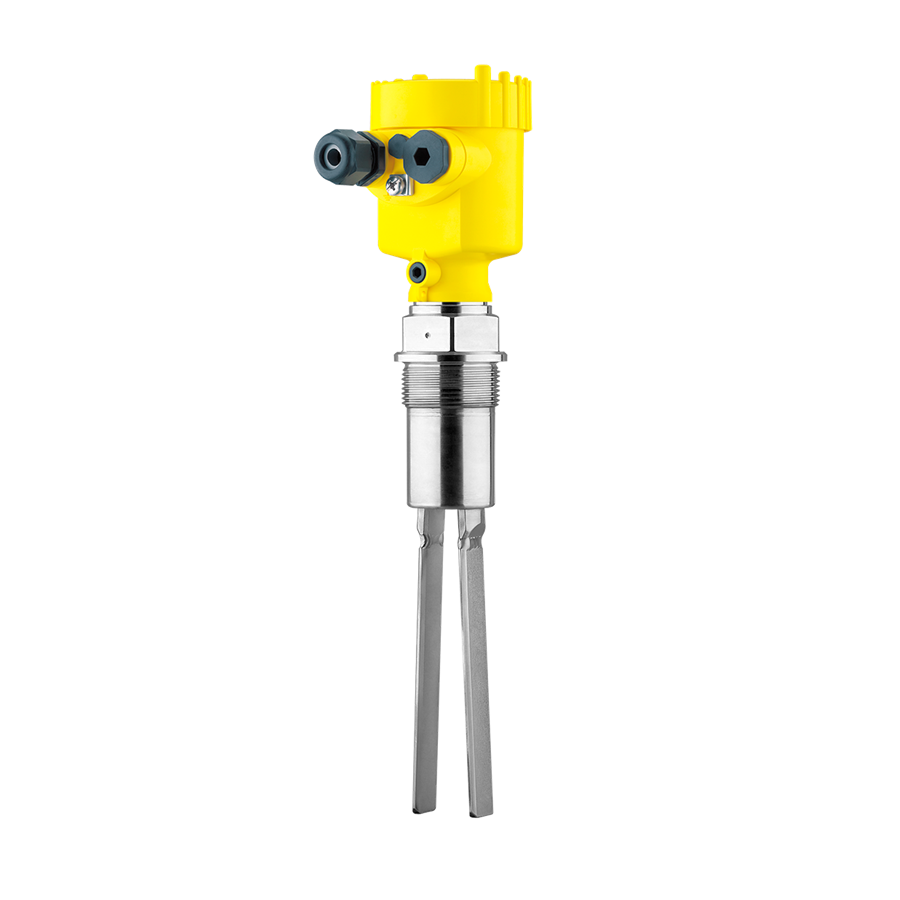
\includegraphics[width = 0.9\linewidth]{fig/Nivel/vibracion.png}\\ \tiny{\href{https://www.secoin.com.uy/productos/}{By: Secoin}}
        \end{column}
        
        \begin{column}{0.50\textwidth}
        \textbf{Detector de vibración}
            \begin{itemize}
                \item Consiste en una sonda de vibración en forma de horquilla que forma parte de un sistema resonante mecánico excitado piezoeléctricamente.
                \item Cuando el material entra en contacto con la sonda amortigua su vibración.
                \item Es adecuado para una gran variedad de polvos, carbon, azúcar, grano, cemento y arena. La exactitud es del ± 1\%.
                
            \end{itemize}
        
        \end{column}
    \end{columns}
\end{frame} 

\begin{frame}{Medidores de nivel de sólidos (punto fijo)}
    \begin{columns}[c, onlytextwidth]
        \begin{column}{0.45\textwidth}
        \textbf{Paletas Rotativas}
            \begin{itemize}
                \item consisten en un eje vertical, dotado de paletas, que gira continuamente a baja velocidad accionado por un motor síncrono.
                \item Cuando el producto sólido llega hasta las paletas, las inmoviliza
                \item Estos aparatos son adecuados en tanques abiertos a baja presión.
                \item Tienen una exactitud de unos ± 25 mm
            \end{itemize}
        \end{column}
        \begin{column}{0.50\textwidth}
        \centering
            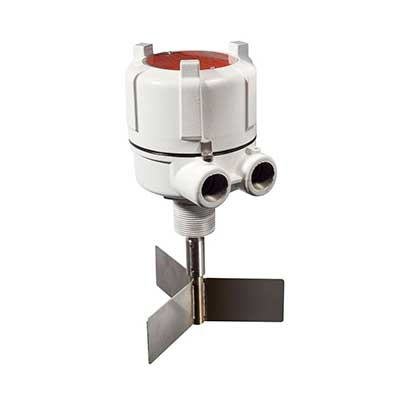
\includegraphics[width = 0.9\linewidth]{fig/Nivel/PaletaRotativa.jpg}\\
            \tiny{\href{https://www.dastecsrl.com.ar/divisiones/caudal-nivel-presion-humedad-y-pesaje/nivel-puntual/paleta-rotativa/bmrx-detector-de-nivel-por-paleta-rotativa-para-solidos}{By: DASTEC}}
        \end{column}
    \end{columns}
\end{frame}

\begin{frame}{Medidores de nivel de sólidos (punto fijo)}
 \begin{table}[]
 \footnotesize
    \centering
    \begin{tabular}{m{3.2cm} m{1.2cm} m{1.6cm} m{1.9cm} m{1.8cm} m{1.6cm}}
        \toprule
        \textbf{Tipo de Sensor} & \textbf{Exactitud [$\%$]} & \textbf{Temperatura [$^{\circ}C$]} & \textbf{Tanque Abierto} &\textbf{Tanque Cerrado}  & \textbf{Precio} \\
        \midrule
        \textbf{Diafragma} & $\pm0.5$ & 60 & \checkmark & \checkmark & Bajo\\
        \textbf{Sonda} & $\pm0.5$  & 60 & \checkmark & X & Bajo\\
        \textbf{Capacitivo} & $\pm0.5$  & 300 & \checkmark & X & Bajo\\
        \textbf{Paletas Rotativas} & $\pm0.5$  & 60 & \checkmark & X & Bajo\\
        \textbf{Vibración} & $\pm1$  & 60 & \checkmark & \checkmark & Medio\\
        \textbf{Radar con haz de luz} & $\pm2$  & 150 & \checkmark & \checkmark & Alto\\
        \bottomrule
    \end{tabular}
    \tiny{\caption{Comparación entre distintos medidores de nivel de solido de punto fijo} \cite{sole2005instrumentacion}}
    \label{tab:Comparacion_sensores_puntoFijo}
\end{table}
\end{frame}

\begin{frame}{Medidores de nivel de sólidos (continuo)}
 \begin{table}[]
 \footnotesize
    \centering
    \begin{tabular}{m{3.2cm} m{1.2cm} m{1.6cm} m{1.9cm} m{1.8cm} m{1.6cm}}
        \toprule
        \textbf{Tipo de Sensor} & \textbf{Exactitud [$\%$]} & \textbf{Temperatura [$^{\circ}C$]} & \textbf{Tanque Abierto} &\textbf{Tanque Cerrado}  & \textbf{Precio} \\
        \midrule
        \textbf{Capacitivo} & $\pm 15mm$ & 150 & \checkmark & \checkmark & Bajo\\
        \textbf{Ultrasónico} & $\pm1$  & 150 & \checkmark & \checkmark & Bajo\\
        \textbf{Radar} & $\pm2$  & 150 & \checkmark & \checkmark & Alto\\
        \textbf{Radiación} & $\pm1$  & 1300 & \checkmark & \checkmark & Alto\\
        \textbf{Laser} & $\pm1$  & 1300 & \checkmark & \checkmark & Alto\\
        \bottomrule
    \end{tabular}
    \tiny{\caption{Comparación entre distintos medidores de nivel de solido continuo} \cite{sole2005instrumentacion}}
    \label{tab:Comparacion_sensores_continuo}
\end{table}
\end{frame}


\begin{frame}{Referencias}
\bibliographystyle{ieeetr}
\footnotesize
\bibliography{comunes/referencias}
\end{frame}

\end{document}